\documentclass[a4paper]{article}
\usepackage[margin=1in]{geometry}
\usepackage[english]{babel}
\usepackage[utf8]{inputenc}
\usepackage{amsmath}
\usepackage{graphicx}
\usepackage{amssymb}
\usepackage{amsthm}
\usepackage{tikz-cd}
\usepackage{mathrsfs}
\usepackage[colorinlistoftodos]{todonotes}
\usepackage{enumitem}
\usepackage{yfonts}
\usepackage{dsfont}
\usepackage{mathtools}
\usepackage{hyperref}
\usepackage{tikz}
\usetikzlibrary{positioning, shapes.geometric, decorations.pathreplacing, calc, backgrounds, through}
\DeclarePairedDelimiter\ceil{\lceil}{\rceil}
\DeclarePairedDelimiter\floor{\lfloor}{\rfloor}

\title{Extremal Combinatorics Notes}
\author{Wilson Pan}
\date{\today}

\newtheorem{thm}{Theorem}[section]
\newtheorem{lem}[thm]{Lemma}
\newtheorem{defn}[thm]{Definition}
\newtheorem{eg}[thm]{Example}
\newtheorem{ex}[thm]{Exercise}
\newtheorem{conj}[thm]{Conjecture}
\newtheorem{cor}[thm]{Corollary}
\newtheorem{claim}[thm]{Claim}
\newtheorem{rmk}[thm]{Remark}

\newcommand{\ie}{\emph{i.e.} }
\newcommand{\cf}{\emph{cf.} }
\newcommand{\into}{\hookrightarrow}
\newcommand{\dirac}{\slashed{\partial}}
\newcommand{\R}{\mathbb{R}}
\newcommand{\C}{\mathbb{C}}
\newcommand{\Z}{\mathbb{Z}}
\newcommand{\N}{\mathbb{N}}
\newcommand{\Q}{\mathbb{Q}}
\newcommand{\LieT}{\mathfrak{t}}
\newcommand{\T}{\mathbb{T}}
\newcommand{\A}{\mathds{A}}
\newcommand{\HG}{\mathcal{H}}
\newcommand{\F}{\mathbb{F}}
\newcommand{\poly}[2]{\text{Poly}_{#1}(#2)}
\newcommand{\gen}[1]{\langle #1 \rangle}
\newcommand{\Hom}{\text{Hom}}
\newcommand{\E}{\mathbb{E}} 
\newcommand{\len}{\text{len}}
\begin{document}

\maketitle

\tableofcontents
\newpage 
\section{Jan 12}

\begin{defn}
    Turan Numbers (Forbidden Subgraph Problems): $F$ is a graph and $G$ graph is $F$-free if $G$ contains no copy of $F$ as a subgraph. \\\\
    We want to maximize the size of $G$ subject to $G$ being $F$-free. Where size=$e(G)=\#$ edges in $G$
\end{defn}
\begin{defn}
    $ex(n,F)=\max \{e(G) | G \text{ is $F$-free and $G$ is $n$-vertex graph}\} $
\end{defn}
\begin{thm}
    Crude Turan's Theorem: If $G$ is $n$-vertex graph, \[
    e(G)=\epsilon {n \choose 2}
    .\] then $G$ contains an independent set of size greater than or equal $\frac{1}{2}\frac{1}{\epsilon}+\frac{1}{2}$\\
    In particular, if $e(G)\geq (1-\epsilon){n \choose 2}$ edges, then $G$ contains a clique on greater than or equal $\frac{1}{2\epsilon}+\frac{1}{2}$ vertices.
    \[
    ex(n,K_t)\leq \left (1-\frac{1}{2t-1} \right ) {n \choose 2}
    .\] 
    \begin{proof}
        Pick $k$ vertices in $G$ at random without replacement. Say we pick $v_1,...,v_k$\\
        For each edge between $v_i$ and $v_j$, delete $v_i$. \\
        Let $X=\#$ deleted vertices\\
        Note: $X\leq e(G[v_1,...,v_k])=:Y$
        \[
        \mathbb{E}[Y]=\sum_{1\leq i\leq j \leq k}\mathbb{P}[v_iv_j\in e(G)]={k \choose 2}\frac{\epsilon {n \choose 2}}{{n \choose 2}}s=\epsilon {k \choose 2}
        .\] 
        Thus, there is a choice of $v_1,...,v_k$ such that $Y\leq \epsilon {k \choose 2}.$ Fix it. 
        Let $\alpha(G)=$ size of largest independent set in $G$ satisfies $\alpha(G)\geq k-Y\geq k-\epsilon {k \choose 2}$
        \[
        \left (k-\epsilon {k \choose 2}\right )'=1+\frac{\epsilon}{2}-\epsilon k
        .\] 
        Set $k=\frac{1+\frac{\epsilon}{2}}{2}+\delta $ for some $|\delta|\leq \frac{1}{2}$.
        \begin{align*}
            \alpha(G)&\geq \frac{1}{\epsilon}+\frac{1}{2}+\delta -\epsilon \left (\left(\frac{1}{\epsilon}+\frac{1}{2}+\delta\right)\left(\frac{1}{\epsilon}-\frac{1}{2}+\delta\right)\right )/2\\
            &=\frac{1}{\epsilon}+\frac{1}{2}+\delta - \epsilon \frac{(\frac{1}{\epsilon}+\delta)^2-\frac{1}{4}}{2}\\
            &=\frac{1}{\epsilon}+\frac{1}{2}+\delta -\epsilon \frac{(1/\epsilon)^2+2 \frac{1}{\epsilon}\delta +\delta^2-\frac{1}{4}}{2}\\
            &=\frac{1}{2}\frac{1}{\epsilon} + \frac{1}{2}+\frac{\frac{1}{4}-\delta^2}{2}\geq \frac{1}{2}\frac{1}{\epsilon} + \frac{1}{2}
        \end{align*}
    \end{proof}
\end{thm}
\begin{rmk}
    Recall: $k$-uniform hypergraph on vertex set $V$ is a subset of \[
    {V \choose k}:= \{e\subseteq V: |e|=k\}
    .\] 
\end{rmk}
\begin{eg}
    In $k$-uniform hypergraph on vertex with $\epsilon {n\choose k}$ edges there is an independent set of size $\geq c_k \frac{1}{\epsilon}^{\frac{1}{k-1}}$
\end{eg}
\begin{thm} Mantel's Theorem: 
    $ex(n,K_3)=\floor{\frac{n^2}{4}}$\\
    More generally, define Turan's graph $T_{n,r}$ to be the $n$-vertex complete $r$-partite graph with part sizes as equal as possible.\\
    Note: $K_{r+1}\not \subseteq T_{n,r}$ because among $r+1$ vertices some pair is in same part. 
\end{thm}

\begin{thm}
    Turan's Theorem: $ex(n,K_{r+1})=e(T_{n,r})$ and furthermore $T_{n,r}$ is the only extremizer.
    \[
    e(T_{n,r})=\left (1-\frac{1}{r} \right ) {n \choose 2}+ O(n) 
    .\]  
    \begin{proof}
        Let $G$ be a graph on $n$ vertices that is $K_{r+1}$-free and has the maximum possible number of edges (an extremizer). We proceed in two steps.\\\\
        Suppose $G$ is not a complete multipartite graph. Then non-adjacency is not an equivalence relation, implying there exist two non-adjacent vertices $x,y$ that do not have identical neighborhoods.\\\\
        Assume $\deg(x)\leq \deg(y)$. Delete $x$ and then clone $y$ to obtain $y'$. The new graph $G'$ has 
        \[
        e(G') = e(G) - \deg(x) + \deg(y) \geq e(G).
        \]
        Also, $G'$ is $K_{r+1}$-free because any copy of $K_{r+1}$ has at most one of $y$ or $y'$ (since they are non-adjacent). If a clique contains $y'$, it can be swapped for $y$ (since $N(y') \subseteq N(y)$), which would imply $K_{r+1}\subseteq G$, a contradiction.\\\\
        Repeating this process transforms $G$ into a complete multipartite graph without decreasing edges. Thus, the extremizer must be a complete multipartite graph.\\
        Since $G$ is $K_{r+1}$-free, it must be $k$-partite with $k \leq r$. To maximize edges, we set $k=r$. Let the parts have sizes $n_1, \dots, n_r$.
        \[
        e(G) = {n \choose 2} - \sum_{i=1}^r {n_i \choose 2}
        \]
        To maximize $e(G)$, we must minimize the subtracted sum of pairs inside the parts. This occurs when $n_i$ are as equal as possible ($|n_i - n_j| \leq 1$). If $n_i \geq n_j + 2$, moving a vertex from part $i$ to part $j$ increases the edge count by $(n_i-1) - n_j > 0$.\\\\
        Thus, the unique extremizer is the balanced complete $r$-partite graph, $T_{n,r}$.
    \end{proof}
\end{thm}
\newpage
\section{Jan 14}

\begin{proof}
    Second proof of Turan's Theorem with induction on $r$.\\
    (Induction Step) Let $x$ be a vertex of largest degree, let $A=N(x)$ be its neighborhood. 
    \[
    B:=V(G)\setminus A
    .\] 
    We have $e(G)=e(A)+e(A,B)+e(B)$ and $A$ is $K_{r-1}$-free so $e(A)\leq e(T_{|A|,r})$\\
    Each vertex in $B$ has $\deg\leq \deg(x)=|A|$\\
    So, \[
    e(A,B)+e(B)\leq \sum_{v\in B}\deg(v)\leq |B||A|
    .\]
    So, \[
    e(G)\leq e(T_{|A|,r})+|A||B|\leq e(T_{n,r})
    .\]
    The right hand side is equal to number of edges in complete r-partite graph with one part of size $|B|$ and other being as equal as possible. \\
    Equality holds iff $B$ is independent and $A$ must be a copy of $e(T_{|A|,r-1})$. Hence $G$ is $T_{n,r}$ for equality to hold.
\end{proof}
\begin{thm}
    Observe that if $F$ is a graph then \[
\frac{ex(n,F)}{{n \choose 2}}\geq \frac{ex(n+1,F)}{{n+1 \choose 2}}
.\] 
\begin{proof}
    Pick $n$ vertices in an $F$-free $(n+1)$ vertex graph $G$ at random without replacement; let $G'$ be the induced graph on these $n$ vertices. 
    \[
    e(G')\leq ex(n,F)
    .\]
    \[
    \mathbb{E}(e(G'))={n \choose 2} \frac{e(G)}{{n+1 \choose 2}}\implies \frac{e(G)}{{n+1 \choose 2}}\leq \frac{ex(n,F)}{{n \choose 2}}
    .\] 
\end{proof}
\end{thm}
\begin{defn}
    \[
    \pi(F):=\lim_{n\to \infty}\frac{ex(n,F)}{{n \choose 2}}
    .\] 
    The Turan density of $F$ is \[
    \pi(K_{r+1})=1-\frac{1}{r}
    .\] 
\end{defn}
\begin{thm}
    Let $F$ be any graph and let $\epsilon>0$. Let $G$ be an $n$-vertex graph. There is a $\delta>0$ such that \[
    e(G)\geq \left( \pi(F)+\epsilon \right) {n\choose 2} \text{ and } n\geq n_0(F,\epsilon)
    .\] 
    then there are at least $\delta n^{|V(F)|}$ copies of $F$. 
    \begin{proof}
        Let $n_0$ be large enough such that $\frac{ex(n_0,F)}{{n_0 \choose 2}}\leq \pi(F)+\frac{\epsilon}{2}.$ Given $n$-vertex $G$ as in theorem. Pick $n_0$ vertices at random without replacement. Let $G'$ be the $n_0$-vertex graph induced on these chosen vertices. \[
        \mathbb{E}[e(G')]=\frac{e(G)}{{n \choose 2}}{n_0 \choose 2}\geq (\pi(F)+\epsilon){n_0 \choose 2}
        .\] 
        Say $G'$ is good if \[
        e(G')\geq \left(\pi(F)+\frac{\epsilon}{2}  \right){n_0 \choose 2}
        .\] 
        \begin{align*}
            \mathbb{E}(e(G'))&\leq \mathbb{P}(G' \text{ is bad})\left (\pi(F)+\frac{\epsilon}{2}\right ){n_0 \choose 2}+\mathbb{P}(G' \text{ is good}){n_0 \choose 2}\\
            &\leq \left(\pi(F)+\frac{\epsilon}{2}\right ){n_0 \choose 2}+\mathbb{P}(G' \text{ is good}) {n_0 \choose 2}
        \end{align*}
        Then $\frac{\epsilon}{2}{n_0 \choose 2}\leq \mathbb{P}(G' \text{ is good}) {n_0 \choose 2}$ so $P(G' \text{ is good})\geq \frac{\epsilon}{2}$\\
        Pick $|V(F)|$ many vertices without replacement inside $G'$, call the subgraph they induce $G''$. So \[
        G\supset G' \supset G''
        .\]
        \[
        \mathbb{P}(G'' \text{ contains } F)\geq \mathbb{P}(G' \text{ is good})\cdot \mathbb{P}(G'' \text{ contains $F$} | G' \text{ is good})\geq \frac{\epsilon}{2}\frac{1}{{n_0 \choose |V(F)|}}
        .\] 
        Note that $G''$ is uniformly randomly chosen $|V(F)|$-vertex subset of $G.$ This implies the \# copies of $F$ in $G\geq \mathbb{P}(G'' \text{contains F}){n \choose |V(F)|}\geq P(...)\frac{n^{|V(F)|}(1-o(1))}{|V(F)|!}.$ We can choose $\delta=\frac{1}{{n_0 \choose |V(F)|}}$ 
    \end{proof}
\end{thm}
\newpage
\section{Jan 16}

\begin{thm}[Erd\H{o}s-Stone-Simonovits]
    Let $T_{n,r}$ denote the Tur\'{a}n graph. We know that:
    \[
    ex(n, T_{s,(r+1)}) = \left (1-\frac{1}{r}+o(1)\right ){n \choose 2}.
    \] 
    This implies that if $H$ is any graph with chromatic number $\chi(H) = r+1$, then
    \[
    ex(n,H) \leq \left( 1-\frac{1}{r}+o(1) \right){n \choose 2}.
    \] 
    Conversely, if $\chi(H) > r$ (i.e., $H$ is not $r$-partite), then $T_{n,r}$ is $H$-free. Hence,
    \[
    ex(n,H) \geq e(T_{n,r}) = \left( 1-\frac{1}{r}+o(1) \right){n \choose 2}.
    \] 
    Combining these, for any non-bipartite graph $H$:
    \[
    ex(n,H) = \left( 1-\frac{1}{\chi(H)-1}+o(1) \right){n \choose 2}.
    \] 
    It is important to note that this theorem holds for bipartite graphs as well, where $\chi(H) = 2$. However, substituting $r = \chi(H) - 1 = 1$ gives a coefficient of $1 - 1/1 = 0$. This implies that $ex(n, H) = o(n^2)$, but it does not provide the precise asymptotic behavior (e.g., $n^{2-\epsilon}$). Therefore, while valid, the Erd\H{o}s-Stone-Simonovits theorem is not the primary tool for determining extremal numbers of bipartite graphs; we rely on theorems like K\H{o}v\'{a}ri-S\'{o}s-Tur\'{a}n for those bounds.
\end{thm}

\begin{thm}[K\H{o}v\'{a}ri-S\'{o}s-Tur\'{a}n 1954]
    \[
    ex(n,K_{s,t}) \leq \frac{1}{2}(t-1)^{\frac{1}{s}}\cdot n^{2-\frac{1}{s}} + O(n).
    \] 
    \begin{proof}
        Let $G$ be a $K_{s,t}$-free graph with $n$ vertices. We will count $X$, the number of copies of $K_{1,s}$ (stars with $s$ leaves).

\begin{center}
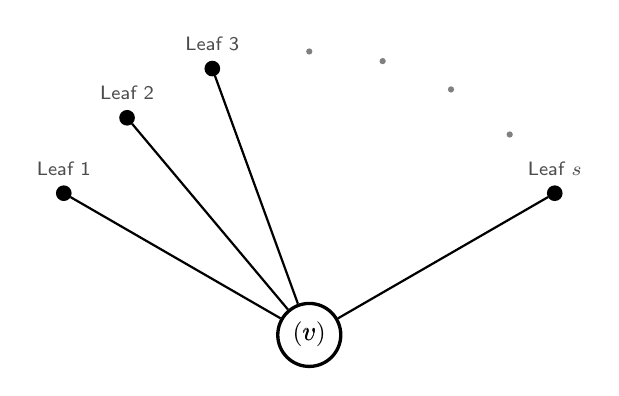
\begin{tikzpicture}[
    % GLOBAL SETTINGS
    scale=1.2,
    thick,
    % STYLES
    root/.style={circle, draw=black, fill=white, very thick, minimum size=8mm, inner sep=0pt},
    leaf/.style={circle, fill=black, inner sep=2pt, outer sep=0pt},
    leaf_label/.style={font=\scriptsize\sffamily, color=black!70},
    edge/.style={draw, thick, -},
    brace/.style={decorate, decoration={brace, amplitude=10pt, raise=5pt}, thick}
]

    \def\radius{3cm}
    \def\startangle{150}
    \def\endangle{30}

    \node[root, label={[yshift=-20pt]\small ($v$)}] (root) at (0,0) {$v$};

    \coordinate (leaf_start) at (\startangle:\radius);
    \coordinate (leaf_end)   at (\endangle:\radius);

    % Draw Leaf 1, Leaf 2, Leaf 3
    \foreach \i/\ang/\lbl in {1/150/1, 2/130/2, 3/110/3} {
        \node[leaf, label={[leaf_label]above:Leaf \lbl}] (l\i) at (\ang:\radius) {};
        \draw[edge] (root) -- (l\i);
    }

    % Draw the last Leaf (Leaf s)
    \node[leaf, label={[leaf_label]above:Leaf $s$}] (ls) at (\endangle:\radius) {};
    \draw[edge] (root) -- (ls);

    \foreach \ang in {90, 75, 60, 45} {
        \node[circle, fill=black!50, inner sep=0.8pt] at (\ang:\radius) {};
    }

\end{tikzpicture}
\end{center}
        We count this in two ways:
        \begin{enumerate}
            \item Since there is no $K_{s,t}$, any set of $s$ vertices can have at most $t-1$ common neighbors. Thus:
            \[ X \leq {n \choose s}(t-1). \]
            \item Let $d_v$ be the degree of vertex $v$. Then:
            \[
            X = \sum_{v\in V(G)}{d_v \choose s}.
            \] 
            A simple-minded application of Jensen's inequality here fails because the binomial coefficient $\binom{x}{s}$ is not convex for all $x$. To fix this, we define the function:
            \[
            f_s(x)=\begin{cases}
                {x \choose s} & \text{if } x\geq s-1\\
                0 & \text{otherwise.}
            \end{cases}
            \]
            Note that $f_s(x)$ is convex for all $x$ because its derivative:
            \[
            \frac{d}{dx}f_s(x)=\begin{cases}
                \left( \frac{1}{x}+\frac{1}{x-1}+\cdots + \frac{1}{x-s+1} \right) { x \choose s} & \text{if } x>s-1\\
                0 & \text{otherwise}
            \end{cases}
            \] 
            is non-decreasing. Since $d_v$ is an integer, $\binom{d_v}{s} = f_s(d_v)$. We can now validly apply Jensen's inequality:
            \[ X = \sum_{v \in V} f_s(d_v) \geq n f_s(d_{\text{avg}}) = n f_s \left( \frac{2m}{n} \right), \]
            where $m=e(G)$. 
        \end{enumerate}
        Combining (1) and (2):
        \[
        n f_s \left(  \frac{2m}{n} \right) \leq {n \choose s}(t-1).
        \]
        If $m \leq \frac{1}{2}(s-1)n$, the bound holds trivially. Otherwise, we approximate ${x \choose s} \approx \frac{x^s}{s!}$:
        \[
        n \frac{\left (\frac{2m}{n}-s\right )^s}{s!} \leq (t-1)\frac{n^s}{s!}.
        \] 
        Rearranging yields:
        \[
        \frac{2m}{n} \leq (t-1)^{\frac{1}{s}} n^{1-\frac{1}{s}} + s \implies m \leq \frac{1}{2}(t-1)^{\frac{1}{s}} n^{2-\frac{1}{s}} + O(n).
        \] 
    \end{proof}
\end{thm}

\begin{eg}[Unit Distance Problem]
    How can we place $n$ points in $\R^2$ to maximize the number of pairs $(p,q)$ such that $||p-q||=1$?\\\\
    A strong construction is a $\sqrt{n}\times \sqrt{n}$ grid. Rather than scaling the grid to unit step size, we scale it such that the distance $1$ corresponds to a distance $d$ in the integer grid that occurs most frequently.\\\\
    The possible distances in an unscaled integer grid are $\sqrt{a^2+b^2}$ for $0 \le a,b < \sqrt{n}$. By number theory (Landau-Ramanujan), integers representable as a sum of two squares are those where primes $p \equiv 3 \pmod 4$ appear with even exponents.\\\\
    To get a better bound, we look for "highly composite" integers. Specifically, if we choose a number $d$ composed of a product of many distinct primes $p \equiv 1 \pmod 4$, the number of ways to write $d$ as a sum of two squares is very large. Erd\H{o}s used this to show there exists a distance occurring:
    \[
    n^{1 + \frac{c}{\log \log n}}.
    \]
    This is significantly larger than the $n\sqrt{\log n}$ bound derived from the Pigeonhole Principle on generic integers.
\end{eg}


\begin{thm}[Upper Bound for Unit Distances]
    The number of unit distances is $O(n^{3/2})$.
    
    \begin{proof}
        Given $n$ points in $\R^2$, construct a graph where vertices are points and $v\sim u$ if $||v-u||= 1$.
        Observe the graph is $K_{2,3}$-free. Geometrically, this is because two circles with radius 1 intersect at most 2 times; thus, no 2 vertices can share 3 common neighbors.\\
        By KST with $s=2, t=3$:
        \[ e(G) \leq \frac{1}{2}\sqrt{3-1} \cdot n^{2-\frac{1}{2}} + o(n^2) = \frac{1}{\sqrt{2}}n^{\frac{3}{2}} + o(n^2). \]
    \end{proof}
\end{thm}

\begin{defn}
    Define $K_{s_1,s_2,t}^{(3)}$ to be the complete $3$-uniform, $3$-partite hypergraph with parts of size $s_1, s_2, t$.
\end{defn}

\begin{thm}[Generalization of KST to Hypergraphs]
    For the $3$-uniform case:
    \[
    ex(n,K_{s_1,s_2,t}^{(3)}) \leq C_{s_1,s_2,t} n^{3-\frac{1}{s_1s_2}} + O(n^2).
    \] 
    \begin{proof}
    We will count the number of stars $K_{1,1,s_1}$ (sets of edges sharing a common pair of vertices). Let $X$ be this number. For any pair $\{v_1,v_2\}$, let $d_{v_1,v_2}$ be the co-degree (number of edges containing $\{v_1,v_2\}$).
    
    \begin{enumerate}
        \item \textbf{Upper Bound on X:} Fix a set $U$ of size $s_1$. Define an auxiliary graph $G_U$ on $V(G)$ where $v_1 \sim v_2$ in $G_U$ if $\{v_1, v_2, u\} \in E(G)$ for all $u \in U$. 
        If $G_U$ contains a copy of $K_{s_2,t}$, then combined with $U$, we form a $K_{s_1,s_2,t}^{(3)}$. Thus, $G_U$ must be $K_{s_2,t}$-free.
        \[
        X \leq {n \choose s_1} ex(n,K_{s_2,t}) \leq C {n \choose s_1} n^{2-\frac{1}{s_2}}.
        \]
        
        \item \textbf{Lower Bound on X:} Summing over pairs:
        \[
        X = \sum_{\{v_1,v_2\}\in {V \choose 2}}{d_{v_1,v_2} \choose s_1} \geq {n \choose 2} f_{s_1} \left( \frac{3m}{{n \choose 2}} \right).
        \]
    \end{enumerate}
    Combining bounds (assuming $m$ is large enough):
    \[
    \binom{n}{2} \frac{\left( \frac{3m}{n^2/2} \right)^{s_1}}{s_1!} \lesssim \frac{n^{s_1}}{s_1!} n^{2-\frac{1}{s_2}}.
    \]
    Simplifying:
    \[
    n^2 \left( \frac{m}{n^2} \right)^{s_1} \lesssim n^{s_1 + 2 - \frac{1}{s_2}} \implies m^{s_1} \lesssim n^{3s_1 - \frac{1}{s_2}}.
    \]
    Taking the $s_1$-th root:
    \[
    m \leq C n^{3-\frac{1}{s_1s_2}}.
    \]
    \end{proof}
\end{thm}
\newpage
\section{Jan 21: Supersaturation and Generalized Turán Problems}

\subsection{Supersaturation}

The classical Turán problem asks for the maximum number of edges in a graph avoiding a subgraph $F$. Supersaturation asks: what happens if we have just \emph{slightly} more edges than this threshold? It turns out we don't just get one copy of $F$, but exponentially many.

\begin{lem}[Supersaturation Lemma]
    If $G$ is a graph on $n$ vertices with $e(G) \geq (\pi(F)+\epsilon)\binom{n}{2}$ edges, then $G$ contains at least $\delta(\epsilon)n^{|V(F)|}$ copies of $F$, where $\delta(\epsilon) > 0$ is a constant independent of $n$.
\end{lem}

\begin{cor}
    For the complete graph $K_{r+1}$, we know $\pi(K_{r+1}) = 1 - \frac{1}{r}$. Thus:
    \[
    e(G) \geq \left( 1-\frac{1}{r}+\epsilon \right)\binom{n}{2} \implies G \text{ contains } \delta(\epsilon)n^{r+1} \text{ copies of } K_{r+1}.
    \]
\end{cor}

\subsection{Hypergraph K\H{o}v\'{a}ri-S\'{o}s-Tur\'{a}n}

We generalize the KST theorem from bipartite graphs to $r$-uniform hypergraphs. We are looking for the Turán number of the complete $r$-partite hypergraph $K_{s_1, \dots, s_r}^{(r)}$. Note that the theorem statement often simplifies the last parameter to $t$.

\begin{thm}[Generalized K\H{o}v\'{a}ri-S\'{o}s-Tur\'{a}n]
    Let $K = K_{s_1,s_2,\ldots,s_{r-1},t}^{(r)}$ be the complete $r$-partite $r$-uniform hypergraph with part sizes $s_1, \dots, s_{r-1}, t$. Then:
    \[
    \text{ex}(n, K) = O_{s,t}\left(n^{r-\frac{1}{s_1 s_2 \cdots s_{r-1}}}\right).
    \] 
    \begin{proof}
        We proceed by induction on the uniformity $r$. The base case $r=2$ is the standard graph KST theorem. Assume the bound holds for $(r-1)$-uniform hypergraphs.\\
        Let $G$ be an $r$-uniform hypergraph with $n$ vertices and $m$ edges. We define a ``hypergraph star'' $K_{1, 1, \dots, s_1}^{(r)}$ as a set of $s_1$ edges that all share a common core of $r-1$ vertices.\\
        Let $X$ be the number of such stars (copies of $K_{1,1,...,1,s_1}^{(r)}$) in $G$. We double count $X$.
        \paragraph{1. Lower Bound (Convexity):}
        For every subset $S \in \binom{V(G)}{r-1}$ of size $r-1$, let the \emph{co-degree} $d_S$ be the number of edges in $G$ containing $S$. A set $S$ contributes $\binom{d_S}{s_1}$ stars to the count.
        \[
        X = \sum_{S\in \binom{V(G)}{r-1}} \binom{d_S}{s_1}.
        \]
        Using Jensen's Inequality (and the convexity of $\binom{x}{s_1}$), we bound this sum:
        \[
        X \geq \binom{n}{r-1} \binom{\bar{d}}{s_1}, \quad \text{where } \bar{d} = \frac{\sum d_S}{\binom{n}{r-1}} = \frac{rm}{\binom{n}{r-1}}.
        \]
        Approximating for large $n$: $\bar{d} \approx \frac{r! m}{n^{r-1}}$ and $\binom{x}{k} \approx \frac{x^k}{k!}$, we get:
        \begin{equation} \label{eq:lower}
            X \gtrsim n^{r-1} \cdot \left( \frac{m}{n^{r-1}} \right)^{s_1}.
        \end{equation}

        \paragraph{2. Upper Bound (Induction):}
        Fix a set of vertices $V_1 = \{v_1, \dots, v_{s_1}\}$. We ask: how many ways can we complete this into a star?\\
        Define an auxiliary $(r-1)$-uniform hypergraph $G_{V_1}$ on $V(G)$. A set $e'$ of size $r-1$ is an edge in $G_{V_1}$ if $e' \cup \{v_i\} \in E(G)$ for all $i=1, \dots, s_1$. In other words, $e'$ is in the common neighborhood of all $v_i$.\\
        If $G_{V_1}$ contains a copy of $K_{s_2, \dots, s_{r-1}, t}^{(r-1)}$, then combined with $V_1$, we would form a copy of the forbidden $K_{s_1, \dots, t}^{(r)}$ in $G$.
        Thus, $G_{V_1}$ must be free of $K_{s_2, \dots, t}^{(r-1)}$. By the inductive hypothesis:
        \[
        e(G_{V_1}) \leq C \cdot n^{(r-1) - \frac{1}{s_2 \dots s_{r-1}}}.
        \]
        Summing over all choices of $V_1$ (there are $\binom{n}{s_1}$ such sets):
        \begin{equation} \label{eq:upper}
            X \leq \binom{n}{s_1} \cdot \max_{V_1} e(G_{V_1}) \lesssim n^{s_1} \cdot n^{r-1 - \frac{1}{s_2 \dots s_{r-1}}}.
        \end{equation}

        \paragraph{3. Conclusion:}
        Comparing \eqref{eq:lower} and \eqref{eq:upper}:
        \[
        n^{r-1} \left( \frac{m}{n^{r-1}} \right)^{s_1} \lesssim n^{s_1 + r - 1 - \frac{1}{s_2 \dots s_{r-1}}}.
        \]
        Rearranging for $m$:
        \[
        m^{s_1} \lesssim n^{(r-1)s_1} \cdot n^{s_1 - \frac{1}{s_2 \dots s_{r-1}}} = n^{rs_1 - \frac{1}{s_2 \dots s_{r-1}}}.
        \]
        Taking the $s_1$-th root:
        \[
        m \lesssim n^{r - \frac{1}{s_1 s_2 \dots s_{r-1}}}. \qedhere
        \]
    \end{proof}
\end{thm}

\subsection{The Erd\H{o}s-Stone Theorem}

\begin{defn}[Blow-up]
    A \textbf{blow-up} of a graph $H$, denoted $H(s)$, is obtained by replacing each vertex $v \in V(H)$ with an independent set $I_v$ of size $s$, and replacing each edge $(u,v) \in E(H)$ with a complete bipartite graph between $I_u$ and $I_v$.\\
    The Turán graph $T_{n,r}$ is essentially a blow-up of $K_r$ with parts of size $n/r$.
\end{defn}

\begin{thm}[Erd\H{o}s-Stone]
    If $e(G) \geq \left( 1-\frac{1}{r}+\epsilon \right)\binom{n}{2}$ and $n$ is sufficiently large, then $G$ contains $T_{s,(r+1)}$ (a blow-up of $K_{r+1}$ with parts of size $s$).\\
    Consequently, $G$ contains any graph $H$ with $\chi(H) = r+1$ (since any such $H$ is a subgraph of a large enough blow-up of $K_{r+1}$).
    \begin{proof}
        \textbf{Step 1: Find many cliques.}
        By the Supersaturation Corollary, since the edge density is greater than the Turán threshold for $K_{r+1}$, $G$ contains many copies of $K_{r+1}$:
        \[
        \# K_{r+1} \geq \delta n^{r+1}.
        \]
        \textbf{Step 2: Construct Auxiliary Hypergraph.}
        Define an $(r+1)$-uniform hypergraph $\mathcal{H}$ with vertex set $V(G)$. Let a set of $r+1$ vertices form an edge in $\mathcal{H}$ if and only if they form a $K_{r+1}$ in the original graph $G$.\\
        From Step 1, we know $e(\mathcal{H}) \geq \delta n^{r+1}$. Since $\delta$ is constant, this is a dense hypergraph.\\
        \textbf{Step 3: Find a dense structure in the hypergraph.}
        We apply the \textbf{Hypergraph KST Theorem} to $\mathcal{H}$. Since $\mathcal{H}$ is dense (order $n^{r+1}$), it exceeds the KST threshold (which is roughly $n^{(r+1) - \epsilon}$).
        Therefore, $\mathcal{H}$ must contain a copy of the complete $(r+1)$-partite hypergraph $K_{s,s,\dots,s}^{(r+1)}$.\\
        \textbf{Step 4: Map back to $G$.}
        Let the parts of this hypergraph copy be $U_1, \dots, U_{r+1}$, each of size $s$. The definition of the complete hypergraph implies that for \emph{any} choice of vertices $u_1 \in U_1, \dots, u_{r+1} \in U_{r+1}$, the set $\{u_1, \dots, u_{r+1}\}$ is an edge in $\mathcal{H}$.\\
        By definition of $\mathcal{H}$, this means $\{u_1, \dots, u_{r+1}\}$ forms a clique $K_{r+1}$ in $G$.
        If every possible tuple forms a clique, then every pair of vertices in distinct parts $U_i, U_j$ must be connected in $G$.\\
        Thus, $G[U_1 \cup \dots \cup U_{r+1}]$ contains the complete multipartite graph with parts of size $s$, which is exactly $T_{s(r+1)}$.
    \end{proof}
\end{thm}

\subsection{Degenerate Turán Numbers (Bipartite Graphs)}

When $H$ is bipartite ($r=1$), the Erd\H{o}s-Stone bound gives $1 - 1/1 = 0$, which is trivial. We rely on KST bounds $ex(n, K_{s,t}) = O(n^{2 - 1/s})$. We examine the sharpness of these bounds.

\begin{thm}[Tightness of KST]
    \hfill
    \begin{enumerate}
        \item \textbf{Case $s=1$ (Trees/Forests):} 
        \[ ex(n, K_{1,t}) \leq \frac{1}{2}(t-1)n. \]
        This is tight for a graph consisting of disjoint copies of $K_t$ (or a matching if $t=1$).
        
        \item \textbf{Case $s=2$ ($C_4$-free graphs):}
        We know $ex(n, K_{2,2}) = O(n^{3/2})$. This is tight.
        
        \textbf{Construction (Finite Geometry):} Let $q$ be a prime power. Construct a bipartite graph $G$ with parts $A$ and $B$, where $|A|=|B|=q^2$.
        \begin{itemize}
            \item Identify vertices in $A$ and $B$ with points in the affine plane $\mathbb{F}_q^2$.
            \item Define edge $(a,b) \sim (x,y)$ if $ax + by = 1$, where $(a,b) \in A$ and $(x,y) \in B$.
        \end{itemize}
        For a fixed vertex $v=(a,b) \in A$, its neighborhood is the set of solutions $(x,y)$ to the linear equation $ax+by=1$. This describes a line in $\mathbb{F}_q^2$, which contains $q$ points (unless $(a,b)=(0,0)$, which we can discard).
        \[
        e(G) \approx q^2 \cdot q = q^3.
        \]
        Since $n = 2q^2$, we have $q \approx \sqrt{n/2}$, so $e(G) \approx (n/2)^{3/2} = \Theta(n^{3/2})$.
        
        \textbf{Why is it $C_4$-free?} A $C_4$ corresponds to two vertices in $A$ sharing two common neighbors in $B$. Geometrically, this means two distinct lines intersect at two distinct points. In a plane, two distinct lines intersect at most at one point. Thus, no $C_4$ exists.
        
        \item \textbf{Case $s=3$ ($K_{3,3}$-free):}
        Tightness $ex(n, K_{3,3}) = \Theta(n^{5/3})$ is known.
        
        \textbf{Construction Sketch:} Vertices are points in $\mathbb{F}_q^3$. Adjacency is defined by $(x,y,z) \sim (a,b,c)$ if $(x-a)^2 + (y-b)^2 + (z-c)^2 = 1$.
        Geometrically, the neighborhood of a point is a unit sphere. If $G$ contained $K_{3,3}$, three vertices in one part would share three common neighbors. This would imply that three unit spheres intersect at three points. In Euclidean geometry, three spheres intersect at most at 2 points (a circle intersects a sphere at 2 points). This logic carries over to $\mathbb{F}_q$ provided $-1$ is not a square.
        
        \item \textbf{Case $s=4$ ($K_{4,4}$-free):}
        It is an \textbf{open problem} whether the KST bound $O(n^{2 - 1/4})$ is tight for $K_{4,4}$.
    \end{enumerate}
\end{thm}

\subsection{Extremal Numbers for Trees}

\begin{lem}
    If a graph $G$ has average degree $d$, it contains a subgraph $H$ with minimum degree $\delta(H) \geq d/2$.
    \begin{proof}
        Let $n = |V(G)|$. We have $e(G) = \frac{dn}{2}$.
        Iteratively delete any vertex with degree strictly less than $d/2$.
        Let $S$ be the set of removed vertices. The number of edges removed is strictly less than $|S| \cdot \frac{d}{2}$.
        Even if we remove $n-1$ vertices, the number of edges removed is $< (n-1)\frac{d}{2} < \frac{dn}{2}$.
        Thus, the edge set cannot be emptied. The process must stop at a non-empty subgraph where every remaining vertex has degree $\geq d/2$.
    \end{proof}
\end{lem}

\begin{thm}
    If $T$ is a tree with $r$ edges (so $r+1$ vertices), then:
    \[
    ex(n,T) \leq rn.
    \]
    \begin{proof}
        Suppose $e(G) > rn$. Then the average degree of $G$ is $d(G) = \frac{2e(G)}{n} > 2r$.
        By the Lemma, there exists a subgraph $H \subseteq G$ with minimum degree $\delta(H) > r$. Since degrees are integers, $\delta(H) \geq r$.
        
        We embed $T$ into $H$ greedily:
        \begin{enumerate}
            \item Order the vertices of $T$ as $v_1, v_2, \dots, v_{r+1}$ such that each $v_i$ (for $i>1$) has exactly one neighbor among $\{v_1, \dots, v_{i-1}\}$. (This is always possible by doing a BFS/DFS from a root).
            \item Map $v_1$ to any vertex $u_1 \in V(H)$.
            \item Suppose we have embedded $v_1, \dots, v_{i-1}$ as $u_1, \dots, u_{i-1}$. Let $v_j$ be the parent of $v_i$ in the tree ($j < i$).
            \item We need to map $v_i$ to a neighbor of $u_j$ in $H$.
            \item The vertex $u_j$ has at least $r$ neighbors in $H$. We have used at most $i-1$ vertices so far. Since $i \leq r+1$, we have used at most $r$ vertices.
            \item We only care that $u_j$ has neighbors not already used in the current tree embedding. The degree of $u_j$ is $\geq r$. The number of currently used vertices is $i-1 \le r$.
            \item The bound requires strict inequality or careful counting. If $\delta(H) \ge r$, $u_j$ has $r$ neighbors. We have used $i-1$ vertices total. If $i-1 < r$, there is space. If $i-1 = r$, we are placing the last vertex. The neighbors of $u_j$ could be occupied by the other $r-1$ vertices of the tree.
            \item However, the conjecture is actually $\frac{1}{2}(r)n$. The bound $rn$ is loose enough. If $e(G) > rn$, avg deg $> 2r$, min deg $\ge r+1$. Then $u_j$ has $r+1$ neighbors, but the tree only has $r+1$ vertices total. At step $i$, only $i-1 \le r$ vertices are occupied. Thus there is always at least one free neighbor for $u_j$.
        \end{enumerate}
    \end{proof}
\end{thm}
\newpage
\section{Jan 23}
\subsection{Turan Number of Cycles and Girth Problem}
\begin{defn}
    If $\mathcal{F}$ is a family of graphs, $ex(n,\mathcal{F})=$ maximum number of edges in an $n$ vertex graph $G$ that contains no $F\in \mathcal{F}$.  
\end{defn}
\begin{lem}
    $ex(n,\mathcal{F})= \left( 1-\frac{1}{r}+o(1) \right){n \choose 2}$ if $r=\min_{{F\in \mathcal{F}}}\mathcal{X}(F)$
    \begin{proof}
        \[
        ex(n,\mathcal{F})\leq \min_{{F\in \mathcal{F}}}ex(n,F)
        .\]
        By Erdos Stone, we're done. 
    \end{proof}
\end{lem}
\begin{thm}
    Let $\mathcal{F}= \{C_{3},...,C_{2k}\}$ then $ex(n,\mathcal{F})\leq n^{{1+\frac{1}{k}}}$
\end{thm}
\begin{lem}
    $G$ is $\mathcal{F}$ free iff $G$ has girth $\geq 2k+1$
\end{lem}
\begin{lem}
    Every graph $G$ contains a subgraph $G'$ that is bipartite with $e(G')\geq \frac{1}{2}e(G)$. 
    \begin{proof}
        Color vertices red or blue uniformly and independent. Then delete the edges that are monochromatic By independence, for any $e\in E(G)$ \[
        \Pr[e\in E(G')]=\frac{1}{2}\implies E[e(G')]=\frac{1}{2}e(G)
        .\] 
    \end{proof}
    \noindent We can also prove this with the greedy algorithm and will achieve a slightly better bound. 
\end{lem}
\begin{proof}
    To prove theorem 5.3:\\
    Suppose $G$ has at least $n^{1+\frac{1}{k}}$, by lemma 5.2 we may replace $G$ by a sub-graph of $\min \deg d\geq n^{1+\frac{1}{k}}$.\\ We can do a depth first search by picking a root vertex $v$. Let $V_{i}$ be the set of vertices at distance $i$ from $v$. So $V_{0}= \{ v\}$ Observe that $G[V_{0},V_{1},...,V_{k}]$ forms a tree with root $v$ and $V_{i}$ being the descendent at at level $i$ else we get a cycle of length at most $2k.$ So we have \[
    |V_{0}|+|V_{1}|+\cdots+|V_{k}|\geq 1+d+(d-1)d+d(d-1)^{2}+\cdots+d(d-1)^{k-1}=1+d^k>n
    .\] 
    So, we have a contradiction.
\end{proof}
\begin{thm}
    $ex(n,C_{2k})\leq c_kn^{1+\frac{1}{k}}$
\end{thm}
\begin{thm}
    $ex(n, \{C_4,C_6,...,C_{2k}\})\leq 2n^{1+\frac{1}{k}}$
\end{thm}
\begin{rmk}
    The exponent $1+\frac{1}{k}$ is sharp if $k=2,3,5$
\end{rmk}
\subsection{Turan Number for Paths} 
\begin{thm}
    Let $P_k$ be a path with $k$ edges then \[
    ex(n,P_k)\leq \frac{k}{2}n
    .\] 
    \begin{proof}
        By induction on $n$ it is enough to work with connected graph as we can just split into connected components. Delete vertices of degree $\leq \frac{k}{2}$. If $e(G)>\frac{k}{2}n$ then this also holds after deletions. So WLOG $G$ has minimum degree at least $\frac{k}{2}$. \\
        Let $v_0,v_1,...,v_r$ be the longest path in $G$. The neighbors of $v_0,v_r$ are in the path otherwise you can extend the path. If $v_0\sim v_r$ then $v_0v_1...v_r$ is a cycle and so $v_iv_{i+1}...v_rv_0...v_{i-1}$ is also a path of same length. Thus, the neighbors of $v_i$ are inside the path. So $ \{v_0,v_1,...,v_r\}$ is a connected conponent of $G$ and thus $v\geq k+1$ else $e(G)\leq \frac{(r-1)n}{2}$. Otherwise, if $v_0 \not \sim v_r$ then there exist $i$ such that $v_0\sim v_{i+1}$ and $v_r\sim v_{i}$ then we can produce a cycle $v_0v_{i+1}v_{i+2}...v_{r}v_{i}v_{i-1}...v_{0}$ and this is of length $r$, so it becomes the previous case. By pigeonhole, such a $i$ exist as $ \{i:v_0v_i+1\in E(G)\}$ and $ \{i:v_rv_i\in E(G)\}$ must intersect as $r\leq k$ by $v_0v_r\notin E(G)$
    \end{proof}
\end{thm}
\newpage
\section{Jan 26: Projective Geometry}

\begin{defn}
    \textbf{Projective Plane over a Field.} Let $\F$ be a field. 
    \begin{enumerate}
        \item \textit{Points:} The set of lines through $0$ in $\F^3$; equivalently, the $1$-dimensional subspaces.
        \item \textit{Lines:} The set of planes through $0$ in $\F^3$; equivalently, the $2$-dimensional subspaces.
        \item \textit{Incidence:} A point $P$ lies on a line $\ell$ if $P \subset \ell$. 
    \end{enumerate}
    Observe:
    \begin{enumerate}
        \item Any two points determine a unique line.
        \item Any two lines intersect in a unique point.
        \item There exist $4$ points no three of which are collinear.
    \end{enumerate}
    Inside a projective plane over $\F$, there is a copy of the affine plane $\F^2$ embedded as $\{z=1\}$.\\
    We denote this by $\mathbb{P}^2(\F)$.\\
    We say $p\sim \ell$ if $p\in \ell$ for $p$ a point and $\ell$ a line of $\mathbb{P}^2(\F_q)$.
\end{defn}

\begin{rmk}
    There are $q^3 - 1$ nonzero vectors in $\F_q^3 \setminus \{0\}$. We identify points of $\mathbb{P}^2(\F_q)$ with equivalence classes of nonzero vectors under
    \[
        (x, y, z) \sim (\lambda x, \lambda y, \lambda z) \quad \text{for } \lambda \in \F_q^\times.
    \]
    There are $q-1$ nonzero choices for $\lambda$, so the number of points in $\mathbb{P}^2(\F_q)$ is
    \[
        \frac{q^3-1}{q-1} = q^2 + q + 1.
    \]
    By a similar argument, the number of lines is also $q^2 + q + 1$.\\
    Each line contains exactly $q + 1$ points and dually, each point lies on exactly $q + 1$ lines. There is a natural bijection (called a \emph{polarity}) between points and lines, preserving incidence: given a point $p$, its corresponding line is the orthogonal complement $p^\perp$.
\end{rmk}

\begin{thm}
    \textbf{Construction of a $C_4$-free graph:}\\
    We construct an improved $C_4$-free graph as follows:
    \begin{itemize}
        \item The vertices are the points of $\mathbb{P}^2(\F_q)$.
        \item Points $p_1$ and $p_2$ are adjacent if and only if $p_1 \in p_2^\perp$ (i.e., $p_1$ lies on the line associated to $p_2$'s orthogonal complement).
    \end{itemize}
    For any pair $p_1, p_2$, their common neighborhood is
    \[
        p_1^\perp \cap p_2^\perp,
    \]
    which is a single point. Thus, the graph is $C_4$-free (contains no $4$-cycles). This gives $q^2+q+1$ vertices with average degree $\approx q$.\\
    Note: There exist $p$ such that $p\subseteq p^\perp$.
\end{thm}

\begin{defn}
    \textbf{General Projective Planes.} If $P$ (points) and $L$ (lines) are sets with an incidence relation such that:
    \begin{enumerate}
        \item For any two points, there is a unique line through them.
        \item Any two lines meet at a unique point.
        \item There exist four points, no three collinear.
    \end{enumerate}
    
    \begin{center}
        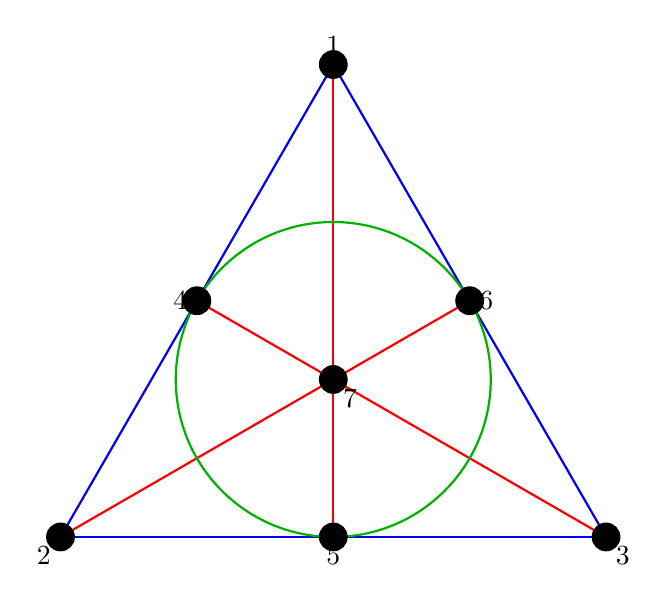
\begin{tikzpicture}[scale=2]
            % 1. Define Coordinates (Equilateral Triangle)
            \coordinate (1) at (90:2);
            \coordinate (2) at (210:2);
            \coordinate (3) at (330:2);
            
            % Midpoints
            \coordinate (4) at (barycentric cs:1=0.5,2=0.5);
            \coordinate (5) at (barycentric cs:2=0.5,3=0.5);
            \coordinate (6) at (barycentric cs:3=0.5,1=0.5);
            
            % Center (Centroid)
            \coordinate (7) at (0,0);
            
            % 2. Draw Lines
            % The 3 outer sides
            \draw[thick, blue] (1) -- (2);
            \draw[thick, blue] (2) -- (3);
            \draw[thick, blue] (3) -- (1);
            
            % The 3 medians (concurrent at point 7)
            \draw[thick, red] (1) -- (5);
            \draw[thick, red] (2) -- (6);
            \draw[thick, red] (3) -- (4);
            
            % The 7th line (the circle through 4, 5, 6)
            \draw[thick, green!70!black] (7) circle (1cm);
            
            % 3. Draw Points
            \foreach \p in {1,2,3,4,5,6,7} {
                \filldraw[black] (\p) circle (2.5pt);
            }
            
            % 4. Labels (slightly offset for clarity)
            \node[above] at (1) {1};
            \node[below left] at (2) {2};
            \node[below right] at (3) {3};
            \node[left] at (4) {4};
            \node[below] at (5) {5};
            \node[right] at (6) {6};
            \node[below right] at (7) {7};
        \end{tikzpicture}
        \end{center}
    \textit{Example: The Fano plane (order 2) with 7 points and 7 lines. Each line contains 3 points, and each point lies on 3 lines.}
\end{defn}


\begin{defn}
    \textbf{Order of a Projective Plane.} The order of a projective plane is the number of points per line minus one (so $q$ if each line has $q+1$ points).
\end{defn}

\begin{rmk}
    Are there planes of order which are not prime powers?
\end{rmk}

\begin{thm}
    \textbf{Construction of $C_{2k}$-free graphs for $k=2,3,5$:}\\
    Let $q$ be a prime power and let $\F_q$ be the finite field with $q$ elements. Define a graph $G$ on the vertex set $\F_q^k$ (the set of $k$-tuples over $\F_q$) as follows:\\
    For $\mathbf{a} = (a_0, a_1, \ldots, a_{k-1})$ and $\mathbf{b} = (b_0, b_1, \ldots, b_{k-1})$ in $\F_q^k$, declare $\mathbf{a} \sim \mathbf{b}$ if and only if for all $j = 0, 1, \ldots, k-2$,
    \[
        b_j = a_j + a_{j+1} \cdot b_{k-1}
    \]
    where indices are taken modulo $k$ (so $a_k = a_0$).\\
    Then $G$ is $C_{2k}$-free, i.e., it contains no cycle of length $2k$.
    \begin{proof}
        Suppose for contradiction that $G$ contains a cycle of length $2k$:
        \[
            \mathbf{a}^1, \mathbf{b}^1, \mathbf{a}^2, \mathbf{b}^2, \ldots, \mathbf{a}^k, \mathbf{b}^k,
        \]
        with $\mathbf{a}^i \sim \mathbf{b}^i \sim \mathbf{a}^{i+1}$ for all $i$, indices modulo $k$.

        \paragraph{Step 1: System of equations.}
        For each $i=1,\ldots,k$ and $j = 0, \ldots, k-2$, adjacency gives:
        \begin{align}
            b_j^i &= a_j^i + a_{j+1}^i \cdot b_{k-1}^i \tag{from $\mathbf{a}^i \sim \mathbf{b}^i$} \\
            b_j^i &= a_j^{i+1} + a_{j+1}^{i+1} \cdot b_{k-1}^i \tag{from $\mathbf{b}^i \sim \mathbf{a}^{i+1}$}
        \end{align}
        Subtract:
        \[
            (a_j^i - a_j^{i+1}) + (a_{j+1}^i - a_{j+1}^{i+1}) \cdot b_{k-1}^i = 0
        \]
        or
        \[
            (a_j^{i+1} - a_j^i) + (a_{j+1}^{i+1} - a_{j+1}^i) \cdot b_{k-1}^i = 0
        \]
        Summing over $i$:
        \[
            \sum_{i=1}^k (a_j^{i+1} - a_j^i) + \sum_{i=1}^k (a_{j+1}^{i+1} - a_{j+1}^i) b_{k-1}^i = 0
        \]
        The first sum telescopes to zero (since indices are cyclic), so for each $j=0,\ldots,k-2$,
        \begin{equation} \label{eq:main}
            \sum_{i=1}^k (a_{j+1}^{i+1} - a_{j+1}^i)\, b_{k-1}^i = 0
        \end{equation}

        \paragraph{Step 2: Specialize $j = k-2$.}
        Let $\triangle_i = a_{k-1}^{i+1} - a_{k-1}^i$ and $x_i = b_{k-1}^i$. Then:
        \[
            \sum_{i=1}^k \triangle_i x_i = 0
        \]
        and
        \[
            \sum_{i=1}^k \triangle_i = 0
        \]
        by telescoping.

        \paragraph{Step 3: Linear algebra.}
        The system \eqref{eq:main} for $j=0,\ldots,k-2$ can be written as a $(k-1) \times k$ Vandermonde-type matrix $V$ applied to the vector $(\triangle_1,\ldots,\triangle_k)$:
        \[
            V = \begin{pmatrix}
                1 & 1 & \cdots & 1 \\
                x_1 & x_2 & \cdots & x_k \\
                x_1^2 & x_2^2 & \cdots & x_k^2 \\
                \vdots & \vdots & & \vdots \\
                x_1^{k-2} & x_2^{k-2} & \cdots & x_k^{k-2}
            \end{pmatrix}
        \]
        The equations become $V \cdot (\triangle_1,\ldots,\triangle_k)^\top = 0$.
        Since $\sum_{i=1}^k \triangle_i = 0$, the vector is in the kernel of the row $(1,1,\ldots,1)$.

        \paragraph{Step 4: Key property of the $x_i$.}
        \begin{claim}
            For each $i$, $x_i \neq x_{i+1}$ (indices modulo $k$).
        \end{claim}
        \begin{proof}
            If $x_i = x_{i+1}$, then $b_{k-1}^i = b_{k-1}^{i+1}$. By the adjacency relations, this forces $\mathbf{b}^i = \mathbf{b}^{i+1}$, so $\mathbf{a}^{i+1} = \mathbf{a}^{i+2}$, contradicting that the cycle is proper.
        \end{proof}

        \paragraph{Step 5: Contradiction for $k=2,3,5$.}
        Since not all $\triangle_i$ are zero (otherwise the cycle is trivial), and $\sum_{i=1}^k \triangle_i = 0$, equation $\sum_{i=1}^k \triangle_i x_i = 0$ forces a linear dependence among the $x_i$ (not all distinct). Thus, for these small $k$ we can classify possibilities:

        \begin{claim}
            For $k=2,3,5$, if $x_i=x_j$ for some $i\neq j$, then $x_i=x_{i+1}$ for some $i$, contradicting the above claim.
        \end{claim}
        \begin{itemize}
            \item \textbf{Case $k=2$:} Only possible if $x_1 = x_2$, violating $x_1\neq x_2$.
            \item \textbf{Case $k=3$:} If $x_1 = x_2$, $x_2 = x_3$, or $x_3=x_1$, we violate the claim.
            \item \textbf{Case $k=5$:} If $x_i = x_j$ for $i\neq j$, by relabeling, could assume $x_1 = x_j$ for $j=2,3,4,5$:
                \begin{itemize}
                    \item $j=2$ or $5$ gives $x_1 = x_2$ or $x_5 = x_1$, directly a violation.
                    \item $j=3$: $x_1 = x_3$. The system $\sum_{i=1}^5 \triangle_i = 0$, $\sum_{i=1}^5 \triangle_i x_i = 0$ with $x_1 = x_3$ and $x_i \neq x_{i+1}$ for any $i$ only allows further coincidences that eventually force $x_i = x_{i+1}$.
                    \item $j=4$: similarly, $x_1 = x_4$ eventually forces a pair $x_i = x_{i+1}$.
                \end{itemize}
            \item \textbf{Case $k=4$:} The pattern $x_1 = x_3 \neq x_2 = x_4$ is possible with no consecutive equal $x_i$, which is why this construction fails for $k=4$.
        \end{itemize}

        Therefore, for $k=2,3,5$, no proper $2k$-cycle exists in $G$.
    \end{proof}
\end{thm}
\newpage
\section{Jan 28}
Recall: $ex(n,K_{s,t})\leq c_{s,t}n^{2-\frac{1}{s}}+o(n)$. We will see that $ex(n,K_{s,t})=\theta \left(  n^{2-\frac{1}{s}} \right)$ for $t\geq t_0(s)$
\begin{thm}
    Construction of the extremal graph for $ex(n,K_{s,t})$. 
    \begin{proof}
        We will first consider a random graph by picking edges with probability $p=n^{-\frac{1}{s}}$. Let $x^{(1)},...,x^{(s)}$ be $s$ vertices chosen uniformly at random without replacement on the left. Let $N(x^{(1),...,x^{(s)}})$ that are the common neighbors with $d(x^{(1)},...,x^{(s)})=|N(...)|$. Let our random variable be $d(x^{(1)},...,x^{(s)})$ and is distributed according to \[
        Binomial(n,p^s)=Binomial\left (n,\frac{1}{n}\right )\sim Poisson(1)
        .\] 
        So $\E[d(x^{(1)},...,x^{(s)})]=1$ and $\E[d(...)^k]=o_k(1)$. With probability $\frac{1}{n^\epsilon}$ there is at least $\epsilon \log n$ neighbors. Yet there are ${n \choose s}$ such $s$ tuples $(x^{(1)},...,x^{(s)})$. and then $\frac{n}{s}$ disjoint. This does not work. \\\\
        Consider another construction of $K_{s,t}$-free graph with $\Omega(n^{2-\frac{1}{s}})$ edges. \\
        For a bipartite graph with $\F_p^s$ where $n=2p^s$ on each side we say $x\sim y$ if $f(x,y)=0$. Pick equation $f$ uniformly at random among all polynomials in $s, t$ of degree at most $d=$ in each of $x$ and $y.$ It would be \[
        f=\sum_{|\alpha|,|\beta|\leq d}c_{\alpha \beta}x_1^{\alpha_1}x_2^{\alpha_2}...x_s^{\alpha_s}y_1^{\beta_1}y_2^{\beta_2}...y_s^{\beta_s} \tag{$c_{\alpha \beta}\in \F_p$, $|\alpha|=\alpha_1+\cdots+\alpha_d$}
        .\] 
        Part I: This random graph is locally (neighborhood look "similar") similar to uniform random graph.\\
        Part II: Globally very different/more discrete. 
    \end{proof}
    \begin{lem}
        For any fixed $x,y\in \F_p^s$ \[
        \Pr[x\sim y]=\frac{1}{p}
        .\] 
        \begin{proof}
            We have \[
                f=c_{0,0}+\sum_{\alpha, \beta\neq 0}c_{\alpha \beta}x^\alpha b^\beta
            .\] 
            For any choice of $c_{\alpha, \beta}$ fir $(\alpha, \beta)\neq (0,0)$ there is a unique choice of $c_{0,0}$ such that $f(x,y)=0.$ \[
            \E[e(G)]=\frac{1}{p}n^2=c_sn^{2-\frac{1}{s}}
            .\] 
        \end{proof}
    \end{lem}
    \noindent Let $x^{(1)},...,x^{(s)}$ be $s$ vertices on say left, $N(x^{(1)},...,x^{(s)})$ be the common neighbors with of $x^{(1)},...,x^{(s)}$ and this is same as $ \{y\in \F_p^s: f(x^{(1)},y)=0,...,f(x^{(s)},y)=0\}$.
    \begin{lem}
        If $g$ is a random polynomial of degree of $D$ in $m$ variables and $z^{(1)},...,z^{(t)}\in \F_p^m$ then the random variables $g(z^{(1)}),...,g(z^{t})$ are independent if $D>t$ and $p>t^2.$
    \end{lem}
    \noindent Warm up: When $m=1$, write $g(x)=\underbrace{a_0+a_1x+\cdots+a_{t-1}x^{t-1}}_{g_\text{small}(x)}+\underbrace{\cdots+a_Dx^D}_{g_\text{large}(x)}$. \\
    For any choice of $g_\text{large}(x)$ and any values $b_1,...,b_t$ there is a unique polynomial $g_{small}$ such that $g(z^{(i)})=g_{small}(z^{(i)})+g_{large}(z^{(i)})=b_i$ for $i=1,...,t$ if and only if $g_\text{small}(z^{(i)})=b_i-g_{large}(z^{(i)})$ by lagrange interpolation.\\\\
    For the general case, if $z_1^{(1)},...,z_1^{(t)},...,z_m^{(1)},...,z_m^{(t)}$ are distinct, then $g(x_1,...,x_m)=\overline{g}(x_1)+$ other terms and use $m=1=$ case. Pick a invertible linear transform $f:\F_p^s\to \F_p^s$ such that $Tz^{(1)},...,Tz^{(t)}$ are distinct. To pick such a $T$, let $T(x_1,...,x_s)=(x_1+S(x_2,...,x_s),x_2,...,x_s)$. For $z^{(i)},z^{(j)}$ distinct, the space of $S$ for which $T(z^{(i)})= T(z^{(j)})$ is of co-dimension $1$, so a random $S$ has probability $\frac{1}{p}$ of satisfying this. So $\Pr[\exists i,j \text{ such that } T(z^{(i)})= T(z^{(j)})]\leq\frac{1}{p}{t \choose 2}<1$.\\\\
    We can now conclude from \[
    \Pr[f(x^{(1)},y)=0,...,f(x^{(s)},y)=0]= \frac{1}{p^s}
    .\] 
    If $d>s$ and $p>s^2$ then \[
    \E[N(x^{(1)},...,x^{(s)})]=1
    .\] \\
    Furthermore, if $\alpha$ is a positive integer and $p \cdot s<d$ then \[
    \E\left [\left |N(x^{(1)},...,x^{(s)}) \right |^p \right] =\E \left [ \left( \sum_{y\in \F_p^s}R(y) \right)^\alpha \right ]=\E \left [\sum_{y^{(1)},...,y^{(\alpha)}} R(y^{(1)})...R(y^{(\alpha)}) \right ]
    .\] 
    Where $R(y)= \begin{cases}
        1 & \text{if } y\in N(x^{(1)},...,x^{(s)})\\
        0 & \text{otherwise}
    \end{cases}$\\
    \[
    =\sum_{y^{(1)},...,y^{(\alpha)}} p^{-s\# \text{distinct y's}} \leq \sum_{k}\sum_{y^{(1)},...,y^{(k)}\in \F_p^s} p^{-sk}=\sum_{k}p^{sk}p^{-sk} \cdot \# \text{ways to partition a objection into $k$ bins}
    .\] 
    Last equality from having to choose $y^{(i)}$ such that $k$ are distinct. This is in $O(1)$. 
    We want to assign values to $y^{(i)}$ such that exactly $k$ are distinct. Equivalently, choose $k$ distinct values in $\F_p^s$. Then choose which of the $y^{(i)}$ go to which bin. 
    \[
    \Pr[|N(x^{(1)},...,x^{(s)})|\geq T] \leq \frac{\E\left [\left |N(x^{(1)},...,x^{(s)}) \right |^\alpha \right ]}{T^\alpha}=\frac{C_{\alpha,s}}{T^\alpha}
    .\] 
    The set $N(x^{(1)},...,x^{(s)})$ is contained in $\{y\in \F_p^s: f(x^{(1)},y)=0,...,f(x^{(s)},y)=0\}$. \\
    A vector subspace $V$ of $\F_p^s$ of dimension $D$ has $p^D$ elements. 
    \begin{thm}
        Lang-Weil Theorem: If $g_1,\ldots,g_r$ are polynomials of degree $\leq D$ in $s$ variables over $\F_p$, then the set $\{y \in \F_p^s : g_1(y) = \cdots = g_r(y) = 0\}$ has either $O_{D,r}(1)$ points, or more than $\frac{p}{2}$ points.
    \end{thm}
    \noindent So $\Pr\left[\text{some $s$ vertices have neighborhood of size} \geq O_{s,\alpha}(1)\right] \leq C_{s,\alpha} \left(\frac{p}{2}\right)^{-\alpha} {p^s \choose s}.$ 
    Choose $\alpha = s^2 + 1$. To ensure this probability goes to $0$, we need to choose $d = s^2 + 1.$
\end{thm}
\newpage
\section{Regularity Lemmas: Feb 4}
\begin{defn}
    Binary word is sequence $w_1,w_2,...,w_n\in \{0, 1\}$ and write $w=w_1w_2...,w_n$.\\
    The density of $w$ is \[
    d(w)=\frac{\# \text{$1$'s in $w$}}{n}
    .\] 
\end{defn}
\begin{defn}
    Word $w$ is $\epsilon$-regular if for any subword $w'$ of $w$ of length $\geq \epsilon \cdot \len(w)$ satisfies \[
    |d(w)-d(w')|\leq \epsilon
    .\] 
\end{defn}
\begin{lem}
    By Chernoff bound, \[
    \Pr[|d(w')-d(w)|\geq \epsilon]\leq e^{-c_\epsilon n}
    .\] 
\end{lem}
\newpage
\section{Feb 6}
\begin{defn}
    Partition $\mathcal{P}'$ is a refinement of partition $\mathcal{P}$ if each $w'\in \mathcal{P}'$ is a sub-word of some word in $\mathcal{P}$  
\end{defn}
\begin{thm}
    (Regularity Lemma for Binary Words)\\
    For all $\epsilon>0$, every word $w\in \{0,1\}^n$ can be partitioned into $\leq M(\epsilon)$ many sub-words $w^{(1)},...,w^{(m)}$ (i.e. $w=w^{(1)}...w^{(m)}$). So that the total length of $w^{(i)}$'s that are $\epsilon$-irregular is at most $\epsilon n.$  
\end{thm}
\begin{proof}
    For a partition $\mathcal{P}$ of $w$ into sub-words $\mathcal{P}= \{w^{(1)},...,w^{(m)}\}$ we define $f(\mathcal{P})=\sum_{w'\in \mathcal{P}}d(w)^2|w'|/|w|$.\\
    Alternatively, we pick a symbol of $w$ at random, say $i\in [n]$ uniformly, then pick another symbol at random from the same part as $1$'st, say $j$ is picked. 
    \[
    \Pr[w_i=w_j]=\sum_{w'\in \mathcal{P}}\frac{|w'|}{|w|}(d(w')^2+(1-d(w'))^2)=2 f(\mathcal{P})+\sum_{w'}\frac{|w'|}{|w|}-2\sum_{w'}d(w')\frac{|w'|}{|w|}=2f(\mathcal{P})+1-2d(w)
    .\] 
    \begin{lem}
        If $\mathcal{P}'$ is a refinement of $\mathcal{P}$ then \[
        f(\mathcal{P}')=f(\mathcal{P})+\sum_{w'\in \mathcal{P}'} \left( d(w')-d(\mathrm{parent}(w')) \right)^2 \frac{|w'|}{|w|}
        .\] 
    \end{lem}
    \begin{proof}
        Expanding the second term we have \[
        \sum_{w'\in \mathcal{P'}}d(w')\frac{|w'|}{|w|}-2d(w')d(\mathrm{parent}(w'))+d(\mathrm{parent}(w'))^2\frac{|w'|}{|w|}=\sum_1+\sum_2+\sum_3
        .\] 
        We have $\sum_1 = f(\mathcal{P}')$ and
        \begin{align*}
        \sum_2 &= \sum_{\tilde{w}\in \mathcal{P}}\sum_{\substack{w'\in \mathcal{P'} \\ \mathrm{parent}(w')=\tilde{w}}} \left( -2d(w')d(\tilde{w})\frac{|w'|}{|w|} \right)\\
        &= \sum_{\tilde{w}\in \mathcal{P}}-2d(\tilde{w})\frac{1}{|w|}\sum_{\substack{w'\in \mathcal{P'} \\ \mathrm{parent}(w')=\tilde{w}}}d(w')|w'|\\
        &= \sum_{\tilde{w}\in \mathcal{P}}-2d(\tilde{w})\frac{1}{|w|} \cdot d(\tilde{w})|\tilde{w}|\\
        &= \sum_{\tilde{w}\in \mathcal{P}}-2d(\tilde{w})^2\frac{|\tilde{w}|}{|w|}\\
        &= -2f(\mathcal{P})
        \end{align*} 
        Then for the third sum 
        \begin{align*}
            \sum_3 &=\sum_{\tilde{w}\in \mathcal{P}}\sum_{\substack{w'\in \mathcal{P'} \\ \mathrm{parent}(w')=\tilde{w}}} d(\tilde{w})^2 \frac{|w'|}{|w|}\\
            &=\sum_{\tilde{w}\in \mathcal{P}}d(\tilde{w})^2 \frac{|\tilde{w}|}{|w|}=f(\mathcal{P})
        \end{align*}
        So we have $\sum_1+\sum_2+\sum_3=f(\mathcal{P}')-f(\mathcal{P})$
    \end{proof}
    \noindent Start with the trivial partition (i.e. $\mathcal{P}= \{w\}$) and repeat while $\sum_{w'\in \mathcal{P} \\ w' \text{ is } \epsilon\text{-irregular}} |w'|\leq \epsilon |w|$.\\
    For $w'\in \mathcal{P}$ that is $\epsilon$-irregular, find a way to write as $w'=w^{(1)}w^{(2)}w^{(3)}$ where $|d(w^{(2)})-d(w^{(1)})|\geq \epsilon$ and $|w^{(2)}|\geq \epsilon |w'|$
    Replace $w'$ with the three words $w^{(1)},w^{(2)},w^{(3)}$ to obtain a new partition of $w$, call it $\mathcal{P}'$. Repeat with $\mathcal{P}$ replaced by $\mathcal{P}'$.\\\\
    To analyze this algorithm, if we drop some words we have \[
    f(\mathcal{P}')\geq f(\mathcal{P})+\sum_{\substack{w'\in \mathcal{P}' \\ w' \text{ is } \epsilon\text{-irregular}}}\sum_{w^{(2)}}(d(w^{(2)}-d(w')))\frac{|w^{(2)}|}{|w|}\geq f(\mathcal{P})+\sum_{\substack{w'\in \mathcal{P}' \\ w' \text{ is } \epsilon\text{-irregular}}}\epsilon^2 \frac{\epsilon |w'|}{|w|}=f(\mathcal{P})+\epsilon^4
    .\] 
    Note: $f(\mathcal{P})\leq 1$ for any partition $\mathcal{P}$.\\
    So the number of steps in the algorithm is $\leq \frac{1}{\epsilon^4}$. The theorem holds with $M(\epsilon)=3^{1/\epsilon^4}$
\end{proof}
\begin{eg}
    Define a twin in a word $w\in \{0,1\}^n$ is a pair of subsequences $x,y\in w$ that are disjoint (no symbol in both $x$ and $y$) and are equal as word. \\
    We define \[
    t(w)=\text{the length of longest pair twins in $w$} \text{ and } t(n)=\min_{w\in \{0,1\}^n} t(w)
    .\] 
    We have the trivial bounds $\frac{n}{4}\leq t(n)\leq \frac{n}{2}$. \\
    \begin{thm}
        \[
        t(n)\geq \left( \frac{1}{2}-o(1) \right)n
        .\] 
    \end{thm}
    \begin{proof}
        Pick small $\epsilon>0$ and cut $w$ into $\epsilon$-regular words $t\leq \epsilon n$ junk symbols. Enough $t(w)\geq \left( \frac{1}{2}-c\epsilon \right)|w|$ for $\epsilon$-regular $w.$\\
        Cut $w$ into $\frac{1}{\epsilon}$ equally long sub-words $w^{(1)},...,w^{(m)}$ where $m=\frac{1}{\epsilon}$. \\
        The first twin is 0's from $w^{(1)}+$ 1's from $w^{(2)}+$ 0's from $w^{(3)}$...\\
        The second twin is 1's from $w^{(1)}+$ 0's from $w^{(2)}+$ 1's from $w^{(3)}$...\\
        Choose twins then \[
        | \text{\# 0's in }w^{(i)}|-| \text{\# 1's in }w^{(2)}|\leq \epsilon |w^{(1)}|
        .\] 
        So, \# symbols not in either of the twins is less than or equal to \[
        \epsilon|w|( \text{1's in } w^{(1)})+\epsilon|w|( \text{1's in } w^{(2)})+\sum_{i}4\epsilon |w^{(i)}|
        .\] 
    \end{proof}
\end{eg}
\newpage
\section{Feb 13}
\begin{defn}
    For disjoint sets $U,V\subset V(G)$, the density between $U$ and $V$ is \[
    d(U,V)=\frac{e(U,V)}{|U|V|}
    .\] 
\end{defn}
\begin{defn}
    A pair $(U,V)$ of disjoint subsets of $V(G)$ is $\epsilon$-regular if $\forall U'\subseteq U, V'\subseteq V$ such that $|U'|\geq \epsilon |U|$ and $|V'|\geq \epsilon |V|$ we have 
    \[
    |d(U,V)-d(U',V')|\leq \epsilon
    .\] 
\end{defn}
\begin{defn}
    We say a partition $V(G)=V_1\cup ...\cup V_k\cup J$ is $\epsilon$-regular partition when
    \begin{enumerate}
        \item $|J|\leq \epsilon |V(G)|$
        \item $|V_1|=|V_2|=...=|V_k|$
        \item All except $\leq \epsilon k^2$ pairs $(V_1,V_2)$ are $\epsilon$-regular 
    \end{enumerate} 
\end{defn}
\begin{thm}
    (Szemeredi's Regularity Lemma) $\forall \epsilon>0,m$ there exist a constant $M=M(\epsilon,m)$ such that every graph admits an $\epsilon$-regular partition $V(G)=V_1\cup \cdots \cup V_K\cup J$ where the number of parts $m\leq K \leq M$. 
\end{thm}
\begin{rmk}
    \# edges inside parts $+$ \# edges adjacent to $J$ $+$ \# edges in $\epsilon$-irregular pairs is at most \[
    k {n/k \choose 2} + (\epsilon n) \cdot n +\epsilon k^2 (n/k)^2\leq \frac{1}{k}n^2+\epsilon n^2+\epsilon n^2
    .\] 
\end{rmk}
\begin{proof}
    For a partition $\mathcal{P}$ of $V:=V(G)$, we define \[
    f(\mathcal{P})=\sum_{U,W\in \mathcal{P}, U \neq W} \underbrace{d(U,W)^2\frac{|U||W|}{|V|^2}}_{f(U,W)}
    .\] 
    \begin{lem}
        Suppose $A,B\subset V$ are disjoint and we have partitions $A=A_1\cup \cdots \cup A_k$ and $B=B_1\cup \cdots \cup B_l$ then \[
        \sum_{i,j}f(A_i,B_j)=f(A,B)+\sum_{i,j} \left( d(A,B)-d(A_i,B_j) \right)^2\frac{|A_i||B_j|}{|V|^2}
        .\] 
        Proof is exactly the same as the proof of the regularity lemma for binary words.
    \end{lem}
    \noindent \textbf{Algorithm}: To find an $\epsilon$-regular partition
    \begin{enumerate}
        \item Start with any equipartition of $V$ into $m$ parts. 
        \item We will start with partitions of the form $V=V_1\cup V_2\cup ...\cup V_k \cup J_1\cup ... \cup J_\ell$ 
        \item For each $\epsilon$-irregular pair $(V_i,V_j)$ there exist partitions $V_i=V_{i,1}^{(i,j)}\cup V_{i,2}^{(i,j)}$ and $V_j=V_{j,1}^{(i,j)}\cup V_{j,2}^{(i,j)}$ such that $|d(V_i, V_j)-d(V_{i,1}^{(i,j)}, V_{j,1}^{(i,j)})|\geq \epsilon$ and $|V_i^{(i,j)}|\leq \epsilon |V_i|$ and $|V_j^{(i,j)}|\leq \epsilon |V_j|$
        \\
        Note: We write is as such since there may be many $\epsilon$-irregular pairs $(V_i,V_j)$ and we want to keep track of them.
        \item For each $i$ consider all partitions of $V_i$ as $V_i=V_{i,1}\cup V_{i,2}$ and take the common refinement. Two $V,V'$ are in the same part of the refinement iff $V,V'$ are in the same part in each of the partitions. \\
        Observe: Each $V_i$ is cut into $\leq 2^k$ parts. \\
        Let $\mathcal{P}$ be the old partition and $\mathcal{P}_{ \text{new}}$ be the new partition.
        \begin{align*}
            f(\mathcal{P}_{ \text{new}})&= \sum_{\substack{A,B\in \mathcal{P}_{ \text{new}}\\ A\neq B}} f(A,B)\\&\geq\sum_i f(J_i, ?)+\sum_{i,j}\sum_{\substack{A,B \\ \text{parent}(A)=V_i \\ \text{parent}(B)=V_j}} f(A,B)\\
            &\geq f( \text{Junk})+\sum_{i\neq j} \left( f(V_i,V_j)+\epsilon^2 \frac{\epsilon^2|V_i||V_j|}{|V|^2} \right)\\
            &=f(\mathcal{P})+\epsilon^4 \left( \frac{|V|-| \text{Junk}}{|V|} \right)^2\\
            &\geq f(\mathcal{P})+\frac{\epsilon^4}{4}
        \end{align*} 
        \item Cut each of the parts in $\mathcal{P}_{ \text{new}}$ into equally big parts so total \# parts is $\leq k\cdot 4^k$ and some left over where \# of leftovers is $\leq k 2^k$ and the size of them $\leq k 2^k \cdot \frac{|V|}{k 4^k}\leq \frac{|V|}{2^k}$\\
        So the total junk size is $\leq \sum_{k\geq m} \frac{|V|}{2^k}$\\
        The total number of iterations is $\leq \frac{4}{\epsilon^4}$ and $g(k)=k 4^k$. The total number of parts at the end is $\leq \underbrace{g(g(\frac{...g}_{4}{\epsilon^4} \text{ times}}(m))...)$
    \end{enumerate} 
\end{proof}
\end{document}